\documentclass[11pt]{article}
\usepackage[margin=1in]{geometry}
\usepackage{mathptmx}
\usepackage{amsmath}
\usepackage{booktabs}
\usepackage{tabularx}
\usepackage{enumitem}
\usepackage{xcolor}
\usepackage{pgfplots}
\usepackage[colorlinks=true,linkcolor=blue!50!black,urlcolor=blue!50!black]{hyperref}
\pgfplotsset{compat=1.17}
\setlist{itemsep=2pt,topsep=3pt}
\newcommand{\verify}[1]{\textcolor{red!70!black}{[VERIFY: #1]}}
\newcommand{\src}[1]{\textcolor{gray}{\small[#1]}}

\title{Montgomery County MPDU Program: Key Provisions}
\author{Summary from the policy documents in \texttt{policy/}}
\date{\today}

\begin{document}
\maketitle

\paragraph{Sources.} Bracketed tags give the source and page.
\begin{itemize}
  \item \textbf{[SR24]} Planning Board staff report, \emph{Overview of the MPDU Program and Designation of 15\% MPDU Planning Areas}, 18 Jan 2024.
  \item \textbf{[ER11-23]} Executive Regulation 11-23 (COMCOR 25A.00.02), effective 7 May 2024: eligibility, rents, HIF payments, resale.
  \item \textbf{[ER21-22]} Executive Regulation 21-22 (COMCOR 25A.00.01), effective 29 Nov 2022: for-sale pricing standards. The file is named \texttt{Exec\_Reg\_21-21}, but the regulation is 21-22.
  \item \textbf{[R04]} Council staff, \emph{Strengthening the MPDU Program: A 30-Year Review}, Feb 2004. Includes Appendix B, a bill-by-bill history.
  \item \textbf{[GIS]} Planning GIS layers in \texttt{data/raw/mcplanning/}: yearly high-income planning-area lists and the 15\% master-plan areas.
\end{itemize}
Two other documents in \texttt{policy/} have little MPDU content. The 2025 pipeline analysis only mentions impact taxes, and \texttt{tax\_reform/Staff\_Report.pdf} covers the FY27 county income and property tax. Items marked \verify{} are not confirmed by these documents.

%==================================================================
\section{Who must provide MPDUs: thresholds}
%==================================================================
\begin{itemize}
  \item \textbf{20+ units:} must provide MPDUs on site. The minimum is 12.5\%--15\% \emph{of the total number of units in the development} (bonus units included). The Planning Board sets the actual number at preliminary or site plan approval. \src{SR24 p.3--4}
  \item \textbf{11--19 units:} no MPDUs are required. Instead, the developer pays the Housing Initiative Fund (HIF):
    \begin{itemize}
      \item for-sale units: 0.5\% of the purchase price of each unit, collected at settlement;
      \item rental units: a comparable amount based on the county's average per-unit sales price over the prior five years, paid before the use-and-occupancy permit;
      \item units added to an existing building that already has controlled MPDUs: the building must designate additional MPDUs instead.
    \end{itemize}
    \src{SR24 p.4; ER11-23 \S3.1}
  \item \textbf{Fewer than 11 units:} no obligation. Developers may provide MPDUs voluntarily and then use the MPDU development standards \src{R04 B-9, Bill 38-02}.
  \item \textbf{The notch at 20 units.} The obligation jumps from 0.5\% of sales value at 19 units to $\lceil 0.125\times 20\rceil = 3$ MPDUs at 20 units.
  \item \textbf{History of the threshold:}
    \begin{itemize}
      \item 1974--2002: 50 or more units \src{R04 B-1}.
      \item From 1 Oct 2002: 35 or more units (Bill 18-02). Projects with 35--49 units were covered only if the site could reach a 20\% bonus, and they were guaranteed at least one bonus market-rate unit \src{R04 9-1, B-9}.
      \item Later: 20 or more units, with the HIF payment for 11--19 units, as in force in 2024. \verify{the year of this change; the 2004 review recommended it (R04 1-5), and it is probably Bill 13-04, effective 2005}.
    \end{itemize}
\end{itemize}

%==================================================================
\section{The minimum share and its geography}
%==================================================================
\begin{itemize}
  \item \textbf{Countywide minimum: 12.5\%.} \src{SR24 p.6}
  \item \textbf{15\% in high-income planning areas (Bill 38-17, effective Oct 2018).} \src{SR24 p.7, 9--12}
    \begin{itemize}
      \item The Planning Board designates these areas every year. A planning area qualifies if at least 45\% of its census-tract acreage has median household income $\geq$ 150\% of the county median, using the latest 5-year ACS.
      \item Tracts are assigned to planning areas by centroid, but the requirement applies within the actual planning-area boundary.
      \item The requirement is fixed when the Planning Board accepts the application as complete.
    \end{itemize}
  \item \textbf{Yearly designations} \src{GIS}:

  \smallskip
  \begin{tabularx}{\linewidth}{@{}lX@{}}
    \toprule
    Year & 15\% planning areas \\
    \midrule
    2019--20 & Bethesda/Chevy Chase, Darnestown, Goshen, Lower Seneca, North Bethesda, Potomac, Travilah, Upper Rock Creek \\
    2021--22 & same, without Goshen \\
    2023 & Bethesda/Chevy Chase, Darnestown, Lower Seneca, North Bethesda, Poolesville, Potomac, Travilah \\
    2024 & Bethesda/Chevy Chase, Darnestown, Lower Seneca, North Bethesda, Potomac, Travilah \\
    2025 & 2024 list + Kemp Mill/4 Corners, Olney, Poolesville \\
    2026 & 2024 list + Dickerson, Olney \\
    \bottomrule
  \end{tabularx}
  \smallskip

    The core (Bethesda/Chevy Chase, Darnestown, Lower Seneca, North Bethesda, Potomac, Travilah) appears every year. Areas at the margin enter and leave, which gives cross-time variation within an area.
  \item \textbf{15\% set by master or sector plans.} Chapter 25A has allowed this since 2018. \src{SR24 p.6--7}
    \begin{itemize}
      \item Bethesda Downtown Plan and Bethesda Overlay Zone (BOZ): 15\% for any project with 20 or more units. Plan approved 24 May 2017 \src{GIS}.
      \item 2022 Silver Spring Downtown and Adjacent Communities (SSDAC) Plan, with the Downtown Silver Spring overlay: 15\% for optional-method projects.
      \item Site-specific example: the Forest Glen Metro parking lot (2020 Forest Glen/Montgomery Hills plan).
      \item Later plans in the GIS layer: Takoma Park minor master plan amendment (2 Apr 2024), University Boulevard Corridor (Dec 2025), Clarksburg Gateway (Mar 2026), Great Seneca (no date in the layer).
      \item Before 2018, some plans made 15\% MPDUs the top-priority public amenity instead, e.g.\ the 2017 Rock Spring Sector Plan.
    \end{itemize}
  \item \textbf{History of the minimum share:}
    \begin{itemize}
      \item 1974: 15\% of units, with a 20\% density bonus \src{R04 3-8, B-1}.
      \item 1981 (Bill 12-80): cut to 12.5\%, bonus still 20\%. The 12.5\% applied to the units planned \emph{before} the bonus, not to the total \src{R04 B-4--B-5}. \verify{when the base switched back to total units, as it is today}.
      \item Until 2001, CBD, Transit Station Residential (TSR) and high-density Planned Development (PD, $\geq$28 du/acre) zones still required 15\% without a sliding scale. Bill 10-01 cut them to 12.5\% and allowed the bonus in CBD optional-method projects \src{R04 3-8, B-8}.
      \item Town Sector and Planned Neighborhood zones once had their own rules (Bills 1-76, 40-78) \src{R04 B-2--B-3}.
    \end{itemize}
\end{itemize}

%==================================================================
\section{The density bonus schedule: kinks and caps}
%==================================================================
\subsection*{Current schedule (Chapter 59, outside the Bethesda Overlay Zone)}
\src{SR24 p.7} With $s$ the MPDU share of total units, the bonus $b$ over mapped residential density is
\[
b(s)=\begin{cases}
0 & s\le 12.5\%\\
8.8\,(s-0.125) & 12.5\% < s\le 15\% \quad\text{(0.88\% per 0.1\%; reaches 22\% at 15\%)}\\
0.22+1.6\,(s-0.15) & 15\% < s\le 20\% \quad\text{(0.16\% per 0.1\%; reaches 30\% at 20\%)}\\
0.30+1.0\,(s-0.20) & s>20\% \quad\text{(0.1\% per 0.1\%)}
\end{cases}
\]
\begin{itemize}
  \item \textbf{No cap on the bonus.} At 100\% MPDUs, $b=110\%$.
  \item \textbf{Kinks} at $s=15\%$ ($b=22\%$) and $s=20\%$ ($b=30\%$). Above each kink, an extra MPDU buys much less density.
  \item \textbf{Date of this schedule.} \verify{that it took effect with the 2014 zoning rewrite (new Chapter 59, District Map Amendment of 30 Oct 2014)}. The 2004 review (below) shows that the earlier schedule stopped at 22\%.
  \item \textbf{In 15\% areas,} public benefit points can still be earned for MPDUs above 12.5\% even though the 15\% is required \src{SR24 p.8}. \verify{the same holds for bonus density, which would make the first 22\% of bonus free in 15\% areas; the simulation (\texttt{rules.py}) assumes it does}.
\end{itemize}

\subsection*{Bethesda Overlay Zone}
\src{SR24 p.9}
\begin{itemize}
  \item The minimum is 15\%.
  \item Bonus density: 17.5\% plus 0.1\% for each 0.1\% of MPDUs above 17.5\%. \verify{whether 15--17.5\% earns any bonus; the text does not say}.
  \item Public benefit points: 15 points per 1\% of MPDUs above 15\%. Projects with at least 20\% MPDUs are excused from most other public benefit categories.
  \item Extra height applies in the Height Incentive Area above 17.5\% MPDUs.
\end{itemize}

\subsection*{1988--2014 schedule (Bill 25-88, with a zoning text amendment)}
\src{R04 10-1, 3-8, B-5}
\begin{itemize}
  \item The table in R04 10-1 (current law in 2004) sets the required share by the bonus achieved:
    \begin{itemize}
      \item no bonus: 12.5\%;
      \item each further 1\% of bonus adds 0.1 points of required MPDUs, up to a 20\% bonus at 14.5\%;
      \item a 22\% bonus requires 15\%.
    \end{itemize}
  \item \textbf{22\% is a hard cap,} reached at 15\%. So 15\% was a corner, not a kink, and there was no tier above 20\%.
  \item The table is in 1\% steps of bonus (``up to 1\%'', ``up to 2\%'', \dots), so strictly it is a step function with small notches. The slope steepens slightly between a 20\% and a 22\% bonus.
  \item Earlier schedules: 1974--1988 had a fixed 20\% bonus and a flat required share (15\%, then 12.5\% from 1981).
  \item In 2004, staff recommended keeping both the 12.5\% minimum and this schedule \src{R04 10-5}. Over half of site plans approved since 1989 used a bonus of 0--5\%, and 23.9\% took the full 22\% \src{R04 10-2}.
\end{itemize}

\begin{figure}[h]
\centering
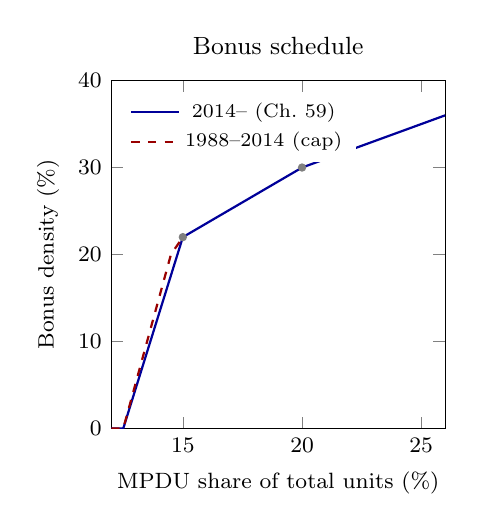
\begin{tikzpicture}
\begin{axis}[width=0.48\linewidth,height=6cm,xmin=12,xmax=26,ymin=0,ymax=40,
  xlabel={MPDU share of total units (\%)},ylabel={Bonus density (\%)},
  title={Bonus schedule},legend pos=north west,legend style={font=\scriptsize,draw=none},
  tick label style={font=\footnotesize},label style={font=\footnotesize},title style={font=\small}]
\addplot[thick,blue!60!black] coordinates {(12,0)(12.5,0)(15,22)(20,30)(26,36)};
\addlegendentry{2014-- (Ch.\ 59)}
\addplot[thick,red!60!black,dashed] coordinates {(12,0)(12.5,0)(14.5,20)(15,22)};
\addlegendentry{1988--2014 (cap)}
\addplot[only marks,mark=*,mark size=1.3pt,gray] coordinates {(15,22)(20,30)};
\end{axis}
\end{tikzpicture}\hfill
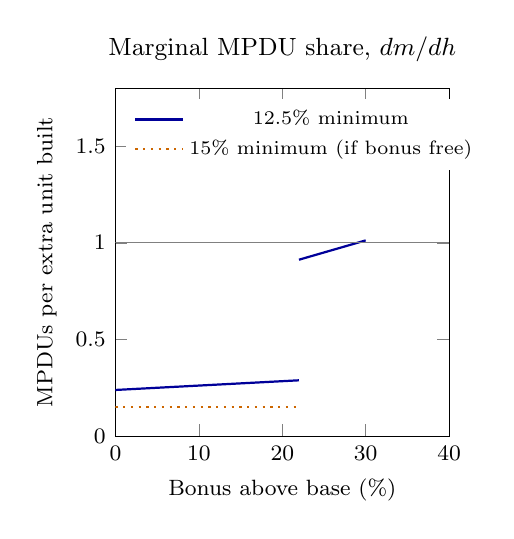
\begin{tikzpicture}
\begin{axis}[width=0.48\linewidth,height=6cm,xmin=0,xmax=40,ymin=0,ymax=1.8,
  xlabel={Bonus above base (\%)},ylabel={MPDUs per extra unit built},
  title={Marginal MPDU share, $dm/dh$},legend pos=north west,legend style={font=\scriptsize,draw=none},
  tick label style={font=\footnotesize},label style={font=\footnotesize},title style={font=\small}]
\addplot[thick,blue!60!black,domain=0:22,samples=20] {(0.125+x/100/8.8)+(1+x/100)/8.8};
\addlegendentry{12.5\% minimum}
\addplot[thick,blue!60!black,domain=22:30,samples=20,forget plot] {(0.15+(x/100-0.22)/1.6)+(1+x/100)/1.6};
\addplot[thick,blue!60!black,domain=30:40,samples=20,forget plot] {(0.20+(x/100-0.30))+(1+x/100)};
\addplot[thick,orange!80!black,dotted,domain=0:22] {0.15};
\addlegendentry{15\% minimum (if bonus free)}
\addplot[gray,thin] coordinates {(0,1)(40,1)};
\end{axis}
\end{tikzpicture}
\caption{Left: bonus density by MPDU share, current schedule and the 1988--2014 schedule (linearized). Right: MPDUs required per extra unit built along the current schedule. Each extra unit raises $h=h_0(1+b)$ and $m=s(b)\,h$, so $dm/dh=s+(1+b)\,s'(b)$. Above 1 (gray line), building more units \emph{reduces} market-rate units. Continuous approximation, ignoring rounding.}
\label{fig:schedule}
\end{figure}

%==================================================================
\section{The implicit tax}
%==================================================================
\begin{itemize}
  \item \textbf{Setup.} Let $k$ be the ratio of MPDU rent to market rent. Then:
    \begin{itemize}
      \item average tax rate: $\text{ATR}=(1-k)\,s$;
      \item marginal tax rate: $\text{MTR}=(1-k)\,dm/dh$.
    \end{itemize}
    The schedule sets $s$ and $dm/dh$. The value of $k$ comes from the rent rules (Section~\ref{sec:prices}) and from market rents. With the \$2,500 placeholder market rent, $k\approx0.6$, so $1-k\approx0.4$.
  \item \textbf{The tax applies from the first unit.} Unlike a pure density-bonus program, the MPDU tax is positive at base density: 12.5\% or 15\% of units, at ATR $\approx0.4\times12.5\%=5\%$. The bonus can only add MPDUs on top of that.
  \item \textbf{Marginal MPDU share along the current schedule,} with a 12.5\% minimum (Figure~\ref{fig:schedule}):
    \begin{itemize}
      \item Tier 1 (bonus 0--22\%): 0.24 rising to 0.29 MPDUs per extra unit. Market-rate units go from $0.875h_0$ to $1.037h_0$.
      \item Tier 2 (bonus 22--30\%): the marginal share jumps to 0.91 and passes 1.0 at $b\approx29\%$ ($s\approx19.4\%$). Market-rate units peak there at $1.040h_0$, only 0.3\% above the 22\% bonus point.
      \item Tier 3 (above a 30\% bonus): 1.5 or more MPDUs per extra unit, so every extra unit built cuts market-rate units. A profit-maximizing developer goes past 20\% MPDUs only if $k$ is close to 1, or for non-density incentives.
    \end{itemize}
  \item \textbf{Implications.}
    \begin{itemize}
      \item With a 12.5\% minimum, the effective decision is whether to use the tier-1 bonus, with a strong prediction of bunching at 15\%/22\%.
      \item With a 15\% minimum, if the first 22\% of bonus is free, bunching at 15\% is mechanical.
      \item Under the 1988--2014 schedule, the marginal share was about 0.23--0.27 up to a 20\% bonus and about 0.45 from 20\% to 22\%, then the cap. Bunching at 15\%/22\% would be a corner solution.
    \end{itemize}
  \item \textbf{Other notches and kinks in the schedule:}
    \begin{itemize}
      \item \emph{20 units:} the jump from the HIF payment to MPDUs (Section 1).
      \item \emph{25\% MPDUs:} school and transportation impact taxes are discounted by the county's lowest rate for that dwelling type, which means a full waiver in infill/red policy areas. Since the 2020 Growth and Infrastructure Policy, the units must be in the MPDU program to qualify \src{SR24 p.8}.
      \item \emph{20\% MPDUs:} meets the entire public benefit requirement for optional-method projects in CR and employment zones. Each 1\% above 12.5\% earns 12 points \src{SR24 p.8}.
      \item \emph{Height:} above 12.5\%, the zone or plan height limit is waived to fit the MPDUs. The allowance is 12~ft per (MPDU floor area above 12.5\% $\div$ average floor plate), with any fraction rounded up to a full floor \src{SR24 p.8}.
      \item \emph{Old 35--49 unit rule (2002--):} the MPDU count was cut if needed to leave at least one bonus market-rate unit \src{R04 9-1}.
    \end{itemize}
  \item \textbf{Rounding} of fractional MPDUs and bonus units is not stated in these documents. \verify{the simulation assumes MPDUs round up and bonus units round down}.
\end{itemize}

%==================================================================
\section{Prices: rents, sales prices, eligibility}\label{sec:prices}
%==================================================================
\subsection*{Income limits}
\src{ER11-23 \S2.2; SR24 p.2--3}
\begin{itemize}
  \item Limits for a household of four:
    \begin{itemize}
      \item 65\% of AMI for rentals in garden apartments, townhouses and single-family homes;
      \item 70\% of AMI for high-rise rentals and all for-sale units.
    \end{itemize}
  \item Other household sizes scale by factors of .70, .80, .90, 1.00, 1.08, 1.16, 1.24 and 1.32 (sizes 1--8), rounded to \$500.
  \item AMI is HUD's figure (\$152,100 in FY2023). If AMI falls, the limits can be frozen or CPI-indexed.
  \item Buyers need at least \$40,000 of income and must not have owned residential property in the past 5 years \src{ER11-23 \S2.4}.
  \item History: a single 65\% limit until the 2004 review, which recommended separate limits for rental and sale units \src{R04 1-3}.
\end{itemize}

\subsection*{Maximum rents}
\src{ER11-23 \S5.2}
\begin{itemize}
  \item Rents are set from the income limit for an implied household size of 1.5 persons per bedroom:
    \begin{itemize}
      \item efficiency: 1 person;
      \item 1BR: 1.5 persons;
      \item 1BR+den: 2 persons;
      \item 2BR: 3 persons;
      \item 2BR+den or 2BR with two baths: 3.5 persons;
      \item 3BR: 4.5 persons.
    \end{itemize}
  \item Monthly rent = 25\% of that income $\div$ 12 if tenants pay utilities, or 30\% if the owner pays all utilities. The result rounds up to a multiple of \$5.
  \item Example: a garden 2BR rent is $0.25\times0.65\times0.90=0.146$ of monthly AMI, and a high-rise 2BR is $0.158$. \verify{these are above the 0.127--0.131 implied by DHCA's current rent list, which \texttt{rules.py} is calibrated to. In-place rents follow the Voluntary Rent Guidelines (\S5.2(e)), not AMI, which may explain part of the gap.}
  \item Rents are fixed when the rental Offering Agreement is approved. Townhouse rents were added in 2024.
  \item Parking: MPDU tenants pay no more than market rate and are never required to rent parking. Surface parking in rental buildings is free.
\end{itemize}

\subsection*{Sales prices: cost-based, not income-based}
\src{ER21-22 \S4--6}
\begin{itemize}
  \item Price = base structure cost (per sq ft by building type: e.g.\ \$107 garden, \$136 mid-rise, \$169 high-rise) + lot development cost + allowed adjustments, plus 30\% for indirect costs and a 3\% closing credit.
  \item Architectural compatibility can add up to 10\%. Buyer options are capped at 10\% of price.
  \item The price is fixed when the Offering Agreement is signed.
  \item Since ER 9-21/21-22, prices are indexed every February to the trailing 5-year average CPI-U (never cut). ER 9-21 raised prices 6.5\%, the first adjustment since 2016.
  \item Impact taxes and WSSC system development charges are waived on MPDUs where the law allows.
\end{itemize}

\subsection*{Unit standards}
\src{ER21-22 \S3}
\begin{itemize}
  \item The MPDU bedroom mix must match the market-rate mix.
  \item No more than 40\% of the units on any floor may be MPDUs.
  \item Minimum unit sizes apply by type. MPDUs need not be on premium floors.
\end{itemize}

%==================================================================
\section{Control periods and resale}
%==================================================================
\begin{itemize}
  \item \textbf{Current terms:} 99 years for rentals, 30 years for for-sale units \src{SR24 p.3}.
  \item \textbf{History:}
    \begin{itemize}
      \item 1974: 5 years for sale and rental units.
      \item 1981 (Bill 12-80): 10 years for both. A 99-year proposal was rejected.
      \item 1989 (Bill 25-88): 20 years for rentals.
      \item From 2002 (Bill 31-01): resale within the control period restarts it.
      \item 2004: the review recommended 99 years for both.
      \item \verify{when today's 30/99 terms were adopted; probably Bill 13-04, effective 2005}.
    \end{itemize}
    \src{R04 3-8, B-4--B-8, 1-3--1-4}
  \item \textbf{Expirations.} Over 2,000 rental MPDUs left control in the 1990s when the 10-year terms expired \src{R04 1-4}. \texttt{10\_dhca\_mpdu\_projects.py} notes that older for-sale units drop out after 10 years.
  \item \textbf{Resale during the control period.} The maximum price is the purchase price + CPI growth + capital improvements (at most 10\% of the price) + broker fee (at most 6\%). DHCA and HOC have a 60-day right of first purchase. Refinancing is capped at the resale price, and reverse mortgages are banned \src{ER11-23 \S8}.
  \item \textbf{First sale after the control period.} Half of the excess over the formula price goes to the HIF. Under the 1988 rule the seller keeps at least \$10,000 \src{ER11-23 \S8.1(b); R04 B-5--B-6}.
\end{itemize}

%==================================================================
\section{Alternatives to on-site MPDUs}
%==================================================================
\src{SR24 p.5--6; ER11-23 \S4}
\begin{itemize}
  \item \textbf{Request timing:} in writing to DHCA at least 90 days before the building permit application and before the Agreement to Build. Approval is at DHCA's discretion.
  \item \textbf{Alternative payment (for-sale only, never rentals):} 3\% of the sales price of every market-rate unit, prorated for any MPDUs provided on site. The developer must show that on-site MPDUs are infeasible.
  \item \textbf{Alternative location (high-rise of 5+ stories, sale or rental):}
    \begin{itemize}
      \item the developer must provide more MPDUs or more bedrooms;
      \item the units must be in the same planning area or in a designated high-income planning area;
      \item existing units may be acquired or rehabilitated.
    \end{itemize}
  \item \textbf{Land transfer:} lots worth at least the value of the MPDUs not built. This option dates to 1974 (Bill 54-73).
  \item \textbf{No alternatives if all impact taxes are waived.}
  \item \textbf{History of buyouts.} Since 1988 (Bill 25-88), HIF payments have been allowed in ``exceptional cases'' with costly bundled fees. DHCA approved 19 buyouts covering more than 230 MPDUs in 2000--2003, mostly height-limited high-rises \src{R04 1-7, 12-3}.
\end{itemize}

%==================================================================
\section{Process and allocation}
%==================================================================
\begin{itemize}
  \item \textbf{Sequence:}
    \begin{itemize}
      \item The Planning Board sets the MPDU count at preliminary or site plan.
      \item The developer signs an Agreement to Build with DHCA before building permits are issued. DPS will not permit the last market-rate unit before the last MPDU \src{ER11-23 \S3.2}.
      \item When the units are ready, the developer signs an Offering Agreement, which fixes the prices.
    \end{itemize}
  \item \textbf{Agency purchase rights.} HOC, DHHS and designated nonprofits can take up to 40\% of offered MPDUs, with HOC up to a third. They have 21 days to choose \src{SR24 p.4}.
  \item \textbf{Remaining for-sale units} go to certificate holders by lottery.
  \item \textbf{Other programs.} MPDUs may be produced under other federal, state or local programs (e.g.\ LIHTC). The MPDU rules then apply for whatever part of the MPDU control period is left after that program's compliance period ends \src{ER11-23 \S3.3}.
\end{itemize}

%==================================================================
\section{Timeline of major changes}
%==================================================================
\small
\begin{tabularx}{\linewidth}{@{}lX@{}}
\toprule
Year & Change \\
\midrule
1974 & Ch.\ 25A (Bill 3-72) takes effect: 50+ units, 15\% MPDUs, 20\% bonus, 5-yr control; HOC option on 1/3; land-transfer option (Bill 54-73). \\
1976 & First MPDUs offered. Income limits tied to metro AMI (Bill 3-76). \\
1981 & Bill 12-80: 12.5\% (of pre-bonus units), 20\% bonus; 10-yr control for sale and rental. \\
1988--89 & Bill 25-88: sliding scale 12.5--15\%, bonus up to 22\%; 20-yr rental control; 50\% of post-control resale windfall to HIF; HIF payment alternative. \\
1994 & Bill 21-94: owner occupancy, staging, bedroom-mix rules. \\
2001 & Bill 10-01: CBD/TSR/PD cut from 15\% to 12.5\%, bonus allowed in CBD. Bill 31-01: control period restarts on resale (sales after Mar 2002). \\
2002 & Bill 18-02 (1 Oct): threshold 50 $\to$ 35 units; 35--49 units guaranteed one bonus market-rate unit. \\
2004--05 & 30-year review. \verify{Bill 13-04: threshold 20, HIF payment for 11--19 units, 30-yr sale / 99-yr rental control.} \\
2014 & \verify{New Chapter 59 (30 Oct 2014): three-tier schedule, kinks at 15\% and 20\%, no cap.} \\
2017 & Bethesda Downtown Plan / Bethesda Overlay Zone: 15\% minimum and a separate bonus schedule. \\
2018 & Bill 38-17 (Oct): 15\% in annually designated high-income planning areas; master plans may set 15\%. \\
2020 & Growth and Infrastructure Policy: 25\% impact-tax waiver requires the units to be MPDUs. \\
2021--22 & ER 9-21 / 21-22: sales prices +6.5\%, then CPI-indexed annually; single 3\% closing credit. \\
2022 & SSDAC Plan: 15\% for optional-method projects in downtown Silver Spring. \\
2024 & ER 11-23: townhouse rental rents; HIF payment formula for 11--19-unit rentals. \\
\bottomrule
\end{tabularx}
\normalsize

\end{document}
